\documentclass[11pt]{article}
\usepackage[T1]{fontenc}
\usepackage{lmodern,microtype}
\usepackage[a4paper,margin=29mm]{geometry}
\usepackage{amsmath,amssymb,amsthm,mathtools}
\usepackage{tikz}
\usetikzlibrary{arrows.meta,positioning,calc}
\usepackage{xcolor,xurl,hyperref}
\hypersetup{colorlinks=true,linkcolor=blue!45!black,citecolor=blue!45!black,
 urlcolor=blue!45!black,
 pdftitle={Exponential PSD rank of positively shifted matching matrices},
 pdfauthor={OpenAI},
 pdfsubject={Positive semidefinite rank, perfect matchings, and exact semidefinite lifts}}
\newtheorem{theorem}{Theorem}[section]
\newtheorem{lemma}[theorem]{Lemma}
\newtheorem{proposition}[theorem]{Proposition}
\newtheorem{corollary}[theorem]{Corollary}
\theoremstyle{definition}
\newtheorem{definition}[theorem]{Definition}
\theoremstyle{remark}
\newtheorem{remark}[theorem]{Remark}
\newcommand{\R}{\mathbb R}
\newcommand{\N}{\mathbb N}
\newcommand{\E}{\mathbb E}
\newcommand{\Id}{I}
\newcommand{\norm}[1]{\left\lVert#1\right\rVert}
\newcommand{\normF}[1]{\left\lVert#1\right\rVert_{\mathrm F}}
\newcommand{\normop}[1]{\left\lVert#1\right\rVert_{\mathrm{op}}}
\DeclareMathOperator{\tr}{tr}
\DeclareMathOperator{\rank}{rank}
\DeclareMathOperator{\rankpsd}{rank_{psd}}
\DeclareMathOperator{\dist}{dist}
\DeclareMathOperator{\supp}{supp}
\numberwithin{equation}{section}
\setlength{\emergencystretch}{1em}
\title{Exponential PSD rank of positively shifted matching matrices}
\author{OpenAI}
\date{October 5, 2026}
\begin{document}
\maketitle
\begin{abstract}
For every fixed $0<\rho<1$, the matrix indexed by odd vertex sets $U$
and perfect matchings $M$ of $K_n$, with entries
$|M\cap\delta(U)|-1+\rho$, has real positive semidefinite rank
$2^{\Omega(n)}$ as even $n$ tends to infinity.  Here $\delta(U)$ is
the edge cut of $U$.  Consequently, every exact semidefinite lift of the
perfect matching polytope has exponential size.
\end{abstract}
\section{Introduction}
\label{sec:introduction}

Semidefinite lifts describe a convex set as the image of an affine
section of a positive semidefinite cone.  They can be substantially
smaller than linear descriptions, so lower bounds for linear extended
formulations do not automatically exclude small semidefinite lifts.
We prove an exponential lower bound for perfect matching by studying
an exact factorization problem that also allows a fixed positive
shift of every odd-cut slack.

For even $n\ge4$, let $E_n$ be the edges of the complete graph $K_n$
on $[n]=\{1,\ldots,n\}$, let $\mathcal M_n$ be its perfect matchings,
and let $\mathcal O_n$ be the odd-cardinality subsets of $[n]$.
For $U\subseteq[n]$, write $\delta(U)$ for the edges with exactly
one endpoint in $U$.  For $0\le\rho\le1$, define the matrix
\begin{equation}\label{eq:main-matrix}
 A_n(\rho)_{U,M}=|M\cap\delta(U)|-1+\rho,
 \qquad U\in\mathcal O_n,\quad M\in\mathcal M_n.
\end{equation}
Every perfect matching crosses an odd set an odd positive number
of times, so this matrix is nonnegative.  Its rows consist solely
of odd cuts.

The \emph{real positive semidefinite rank} of a finite nonnegative
matrix $A$, denoted $\rankpsd A$, is the least integer $r\ge1$ for
which there are real symmetric positive semidefinite matrices
$F_U,G_M\in\R^{r\times r}$ satisfying
\[
 A_{U,M}=\tr(F_UG_M)
 \qquad\text{for every row and column}.
\]
Such matrices are called PSD factors.  The entries must be reproduced
exactly, and no symmetry, equivariance, sparsity, or precision
restriction is imposed on the factors.

\begin{theorem}\label{thm:main}
There is a constant $c>0$ such that, for every fixed $0<\rho<1$,
there is $n_0=n_0(\rho)$ for which
\[
 \rankpsd A_n(\rho)\ge2^{cn}
\]
for every even $n\ge n_0$.
\end{theorem}

The endpoint $\rho=1$ has a factorization of size $\binom n2$:
use diagonal matrices indexed by edges, with diagonal entries
$\mathbf1_{\{e\in\delta(U)\}}$ for a row and
$\mathbf1_{\{e\in M\}}$ for a column.  Thus the endpoint $\rho=1$
cannot be included in the exponential lower bound.
The exponential rate in Theorem~\ref{thm:main} is independent of
$\rho$, although the threshold is allowed to deteriorate as
$\rho$ tends to one.

\subsection{Exact semidefinite lifts}

Let
\[
 P_n=\operatorname{conv}\{\mathbf1_M:M\in\mathcal M_n\}
 \subseteq\R^{E_n}
\]
be the perfect matching polytope.  A \emph{semidefinite lift of
size $r$} represents $P_n$ as an affine image of
$L\cap\mathbb S_+^r$, where $L$ is an affine subspace of the real
symmetric matrices and $\mathbb S_+^r$ is their PSD cone.  Also let
$T_n(\rho)$ denote the matrix obtained by adjoining to $A_n(\rho)$
the edge rows
\[
 T_n(\rho)_{e,M}=\mathbf1_{\{e\in M\}},\qquad e\in E_n.
\]
Adding rows cannot decrease PSD rank, so
Theorem~\ref{thm:main} applies to $T_n(\rho)$ as well.

\begin{corollary}[Unshifted rank and exact lifts]
\label{cor:exact-lift}
There are constants $c_0>0$ and $n_1$ such that, for every even
$n\ge n_1$, both $A_n(0)$ and $T_n(0)$ have real PSD rank at least
$2^{c_0n}$, and every exact semidefinite lift of $P_n$ has size at
least $2^{c_0n}$.
\end{corollary}
\begin{proof}
Appending scalar blocks $\rho$ to the row factors and $1$ to the
column factors of $A_n(0)$ gives a factorization of $A_n(\rho)$.
Consequently
\[
 \rankpsd A_n(\rho)\le\rankpsd A_n(0)+1.
\]
Fix $\rho=1/2$ and apply Theorem~\ref{thm:main}.  For all sufficiently
large even $n$,
\[
 \rankpsd T_n(0)\ge\rankpsd A_n(0)\ge2^{cn}-1\ge2^{cn/2}.
\]

Edmonds's description of $P_n$ uses nonnegativity and odd-cut
inequalities, within the affine space of degree equations
$\sum_{e\ni v}x_e=1$ \cite{edmonds}.  Thus $T_n(0)$ is a slack
matrix of this description.  Every row inequality is tight at some
perfect matching.  Any redundant row is therefore a nonnegative
combination of facet slack rows, so including it does not change
PSD rank.  The cone-factorization theorem identifies this rank with
the minimum size of a semidefinite lift
\cite[Theorem~2.4 and Corollary~2.6]{gpt}.

For completeness, an arbitrary lift can be restricted to the
smallest face of the PSD cone containing its feasible section.
This face is a PSD cone of size at most $r$, and the section meets
its relative interior, supplying the properness needed for
factorization.  An affine image can be made linear on the affine
slice without increasing size: the slice cannot contain zero,
since its intersection with the cone would then have a bounded
affine image only if that image were a point.  A linear functional
equal to one on the slice therefore absorbs the translation.
Taking $c_0=c/2$ proves the corollary.
\end{proof}

\subsection{History and the role of the shift}

Edmonds's inequality description \cite{edmonds} is the starting
point for formulation complexity of matching.  Yannakakis
developed the nonnegative-factorization framework and proved an
exponential lower bound for symmetric linear formulations
\cite{yannakakis}.  Rothvo\ss\ proved the unrestricted exponential
linear extension-complexity bound \cite{rothvoss}.  The
cone-factorization framework of Gouveia, Parrilo, and Thomas
\cite{gpt} gives the corresponding connection between PSD rank
and semidefinite lifts.

For the particular shifted matrix, Braun and Pokutta proved
exponential nonnegative rank for the entries
$(|M\cap\delta(U)|-1+\rho)/2$, for each fixed $0<\rho<1$
\cite[Section~2.2.3 and Theorem~3.1]{braun-pokutta}.
Positive scalar multiplication does not change rank, so their
matrix is the same factorization problem with nonnegative scalar
factors in place of arbitrary PSD factors.  Braun and collaborators
proved exponential lower bounds for coordinate-symmetric
semidefinite formulations of matching
\cite[Definition~2.2 and Theorem~3.10]{matching-symmetric}.
Here no group action on the factor coordinates is assumed.
Permutation symmetry will be used only to analyze averaging
operators.

Lee, Raghavendra, and Steurer developed a general approach to
unrestricted SDP lower bounds through sums of squares and
low-degree separating functionals \cite{lrs}.  Our proof follows
that approach, with a transfer argument tailored to matching.
It treats the exact positive shift in Equation~\eqref{eq:main-matrix}.
Exactness matters: Kaniewski, Lee, and de Wolf construct matrices
of subexponential PSD rank that approximate the unshifted matching
slack with entrywise error at most $2^{-\sqrt{n/2}}$
\cite[Section~7.3 and Theorem~19]{kaniewski-lee-dewolf}.

\subsection{Proof strategy and reusable ingredients}

The obstruction is an inconsistent parity system on an expanding
graph $H$ with $t$ vertices.  Each vertex carries $d$ incidence
bits of prescribed parity, and the sum of the prescribed parities
is odd.  Some edge must therefore have unequal bits at its two
ends.  Subtracting $1-\rho$ from the number of disagreements gives
a positive function $f$.  Products of signs of the free incidence
bits give Fourier characters, each involving certain vertex blocks.
Section~\ref{sec:parity} constructs a linear functional that is
nonnegative on squares of functions whose Fourier characters each
involve at most a small fixed fraction of the blocks, yet takes
value $-(1-\rho)$ on $f$.  The signed
moment construction is related to Grigoriev's low-degree
functionals for Tseitin contradictions \cite{grigoriev}.

To realize this system in matching, replace every vertex of $H$
by a cell of $k$ vertices.  The cell size $k$ is a sufficiently
large constant, fixed before $n$ tends to infinity.  Each auxiliary
incidence uses one terminal; the remaining vertices are paired
inside the cell.  A local cut restriction fixes the terminal bits
and gives equal bits to every internal pair.  The only crossing
edges are then the auxiliary disagreements.  Section~\ref{sec:matching}
performs this construction and completes the proof.

The main analytic task is to show that a small PSD factorization
would make $f$ close enough to a low-degree sum of squares.
Let $\overline F(y)$ be the row factor averaged over cuts with
incidence assignment $y$.  Pairing this average with the factor of
the corresponding matching gives $f(y)$.  Taking square roots of
the row factors gives matrix functions with no initial degree bound;
averaging their squares cannot be replaced by squaring their
averages.  We instead construct an exact representation
\[
 \overline F(y)=\sum_q H_q(y)^{\mathsf T}H_q(y)
\]
by real rectangular matrix functions.  The index $q$ labels both
a summand, called a branch, and a Fourier character $\chi_q$.
The goal is to concentrate the coefficients of $H_q$ on characters
that differ from $\chi_q$ in only a few vertex blocks.

Section~\ref{sec:local} proves the local averaging estimate used
at each step.  Its scalar variance bound tends to zero as $k$
grows and extends to matrices without a dimension factor.
The proof combines a trace estimate with a lower bound on the
dimensions of invariant eigenspaces, a spectral mechanism also
used in quasirandom-group arguments \cite{gowers}.
Section~\ref{sec:splitting} proves a dimension-free orthogonal
splitting inequality for a finite family of PSD matrices.

These ingredients yield the abstract product averaging theorem
in Section~\ref{sec:fourier}.  It bounds the Fourier mass of each
branch with weights growing exponentially in the number of blocks
where a character differs from its center $q$.  The controlled quantity is
the squared Frobenius norm of a weighted Gram matrix, hence a
fourth-order expression in the Fourier coefficients.  Its use
allows repeated averaging even though representing an average by
a direct sum introduces additional rows into the matrices $H_q$.
After truncation near the center $q$, multiplication by $\chi_q$
moves each retained character to low block degree while
preserving squares, as in finite-group Fourier sums of squares
\cite{fsp-sparse}.  This is the step that lets the separating
functional contradict the factorization.

The local averaging lemma, the orthogonal splitting inequality,
and the product theorem are stated separately from the global
matching factorization problem.
Appendix~\ref{sec:matching-smoothing} gives a further independent
smoothing theorem for averages over matchings with any prescribed
edge-count table across a fixed number of cells.  Its estimate is
uniform even for rare tables and unbalanced cell sizes, and its
three-cell specialization includes a single polynomial in the
three intercell counts.

\paragraph{Notation.}
Finite sets carry uniform probability unless another law is specified;
averages are denoted by $\E$.  For real matrices we use the Frobenius
norm $\normF B=(\tr(B^{\mathsf T}B))^{1/2}$ and operator norm
$\normop B$.  The relation $A\preceq B$ means that $B-A$ is PSD.
All logarithms are natural unless their base is displayed.

\section{Averaging within a cell}
\label{sec:local}

We next construct restrictions of a cut to one cell.  The restrictions
prescribe its values at a fixed number of terminals and make its values
equal across every internal matching edge.  Averaging a function over
these restrictions has a uniform marginal and, as the cell grows, small
variance over the choice of terminals and matching.  The variance bound
will hold for matrix-valued functions with a constant independent of their
dimensions.

Fix an even integer $d\ge 2$, and let $k$ be a sufficiently large even
integer.  A cell has vertex set $[k]$.  For $b\in\{0,1\}$, let $w$ be the
unique integer in $\{k/2,k/2+1\}$ congruent to $b$ modulo two, and set
\[
  X=\binom{[k]}{w},
  \qquad
  Y_b=\left\{y\in\{0,1\}^d:
       \sum_{\ell=1}^d y_\ell\equiv b\pmod 2\right\},
  \qquad L=|Y_b|=2^{d-1}.
\]
We identify a subset $a\in X$ with its indicator function when referring
to its bits.

Local column data $m$ consist of an ordered list of distinct terminals
$(v_1,\ldots,v_d)$ and a perfect matching of the remaining $k-d$ vertices.
Let $\mathcal M$ be the finite set of these data, with its uniform law.
For $y\in Y_b$, define $\pi_y^m$ to be the uniform probability measure on
the subsets $a\in X$ satisfying
\begin{equation}
  \mathbf 1_a(v_\ell)=y_\ell\quad(1\le\ell\le d),
  \qquad
  \mathbf 1_a(u)=\mathbf 1_a(v)
       \quad\text{for every internal pair }\{u,v\}\text{ of }m.
  \label{local:restrictions}
\end{equation}
To see that this measure is defined, write
\begin{equation}
  s=|y|,\qquad h=\frac{k-d}{2},\qquad
  g=\frac{w-s}{2}.
  \label{local:parameters}
\end{equation}
The parity condition makes $g$ integral.  A subset satisfying
\eqref{local:restrictions} consists of the prescribed terminals and a
choice of $g$ whole pairs among the $h$ internal pairs.  If
$\delta=w-k/2\in\{0,1\}$, then
\begin{equation}
  g=\frac h2+\frac d4+\frac\delta2-\frac s2,
  \qquad
  \left|g-\frac h2\right|\le\frac d4+\frac12.
  \label{local:central}
\end{equation}
Thus $0\le g\le h$ for all sufficiently large $k$, uniformly in $b$ and
$y$.  The support of $\pi_y^m$ has cardinality $\binom hg$.

For a real function $B$ on $X$, define
\[
  (T_yB)(m)=\sum_{a\in X}\pi_y^m(a)B(a).
\]
The same definition applies entrywise to a real matrix-valued function.
Expectations over $a$ and $m$ below use the uniform laws on $X$ and
$\mathcal M$, respectively.

\begin{lemma}[Local averaging]
\label{lem:local-averaging}
For each fixed even $d\ge2$, there are $k_0(d)$ and numbers
$\theta_d(k)\ge0$, defined for even $k\ge k_0(d)$, with
$\theta_d(k)\to0$ as $k\to\infty$, such that the following holds for the
construction above, for both $b\in\{0,1\}$ and every $y\in Y_b$.
First,
\begin{equation}
  \E_m\pi_y^m(a)=\frac1{|X|}\qquad(a\in X).
  \label{local:marginal}
\end{equation}
Second, every real function $B:X\to\R$ satisfies
\begin{equation}
  \E_m\left|(T_yB)(m)-\E_aB(a)\right|^2
  \le\theta_d(k)\,
      \E_a\left|B(a)-\E_aB(a)\right|^2.
  \label{local:scalar-variance}
\end{equation}
For every pair of positive integers $p,q$, the same constant gives, for
every $B:X\to\R^{p\times q}$,
\begin{equation}
  \E_m\normF{(T_yB)(m)-\E_aB(a)}^2
  \le\theta_d(k)\,
      \E_a\normF{B(a)-\E_aB(a)}^2
  \le\theta_d(k)\,\E_a\normF{B(a)}^2.
  \label{local:matrix-variance}
\end{equation}
One may take $\theta_d(k)=O_d(k^{-1/4}\sqrt{\log(k+2)})$.
\end{lemma}

\begin{proof}
The uniform law of $m$ and the restrictions
\eqref{local:restrictions} are equivariant under permutations of the
$k$ vertices.  Since the symmetric group is transitive on $X$, the
marginal law of $a$, obtained by first sampling $m$ and then
$a\sim\pi_y^m$, is uniform.  This proves \eqref{local:marginal}.

Fix $b$ and $y$, and write $T=T_y$.  Equip the function spaces on $X$
and $\mathcal M$ with the inner products for uniform probability, and
put $K=T^*T$.  This is a positive semidefinite self-adjoint operator.
The marginal identity gives $K1=1$.  We will show that
$\tr(K^2)=o(k)$, while every nonconstant eigenspace has dimension at
least $k/2$.  Together these estimates force the largest eigenvalue
on the orthogonal complement of the constants to tend to zero.

\emph{The two-sample kernel.}
Sample $m$ uniformly, and then sample $a,a'$ independently from
$\pi_y^m$ conditional on $m$.  Let $J(a,a')$ be their joint
probability, and let $N=|X|$.  The density of this joint law relative
to two independent uniform elements of $X$ is
$D(a,a')=N^2J(a,a')$.  Indeed, for scalar functions $B_1,B_2$,
\[
  \langle B_1,KB_2\rangle
   =\sum_{a,a'\in X}J(a,a')B_1(a)B_2(a').
\]
Consequently the ordinary matrix entries of $K$ are $D(a,a')/N$, and
symmetry gives
\begin{equation}
  \tr(K^2)=\frac1{N^2}\sum_{a,a'\in X}D(a,a')^2.
  \label{local:density-trace}
\end{equation}

The joint law is permutation-invariant, so $D(a,a')$ depends only on
$|a\cap a'|$.  Conditional on $m$, the two subsets choose independent
$g$-subsets of the $h$ internal pairs.  If the second choice replaces
exactly $j$ pairs of the first, their intersection has size
$s+2(g-j)=w-2j$.  The probability of this event is
\[
  P_j=\frac{\binom gj\binom{h-g}j}{\binom hg},
  \qquad 0\le j\le g_*:=\min(g,h-g).
\]
For two independent uniform elements of $X$, the probability of the
same intersection size is
\[
  Q_j=\frac{\binom w{2j}\binom{k-w}{2j}}{\binom kw}.
\]
Both laws are uniform within each intersection class.  The density
there is therefore $P_j/Q_j$, and it vanishes on the remaining
classes.  The identities
$w=2g+s$ and $k-w=2(h-g)+(d-s)$ ensure that every displayed $Q_j$
is positive.  Equation~\eqref{local:density-trace} becomes
\begin{equation}
  \tr(K^2)
   =\sum_{j=0}^{g_*}\frac{P_j^2}{Q_j}
   =\frac{\binom kw}{\binom hg^2}
      \sum_{j=0}^{g_*}
      \frac{\binom gj^2\binom{h-g}j^2}
           {\binom w{2j}\binom{k-w}{2j}}.
  \label{local:trace-formula}
\end{equation}

\emph{A trace estimate.}
Since $k=2h+d$, $w=k/2+O(1)$, and
$g=h/2+O_d(1)$, the central binomial estimates give
\begin{equation}
  \frac{\binom kw}{\binom hg^2}=O_d(\sqrt h),
  \label{local:central-ratio}
\end{equation}
uniformly in $b$ and $y$.  Moreover,
$\binom w{2j}\ge\binom{2g}{2j}$ and
$\binom{k-w}{2j}\ge\binom{2(h-g)}{2j}$.
For integers $0\le j\le u$, the identity
\[
  \frac{\binom uj^2}{\binom{2u}{2j}}
  =\frac{\binom{2j}j\binom{2(u-j)}{u-j}}{\binom{2u}u}
\]
and the bounds $\binom{2v}v\asymp4^v/\sqrt{v+1}$ imply
\begin{equation}
  \frac{\binom uj^2}{\binom{2u}{2j}}
   \le C\sqrt{\frac{u+1}{(j+1)(u-j+1)}}
  \label{local:binomial-ratio}
\end{equation}
with an absolute constant $C$, including at the endpoints $j=0,u$.
Applying this bound with $u=g$ and $u=h-g$ shows that the sum in
\eqref{local:trace-formula} is at most
\[
  C^2\sum_{j=0}^{g_*}
    \frac{h+1}{(j+1)(g_*-j+1)}
  =\frac{2C^2(h+1)}{g_*+2}\sum_{j=1}^{g_*+1}\frac1j.
\]
By \eqref{local:central}, $g_*=h/2+O_d(1)$, so this is
$O_d(\log(h+2))$.  Thus
\begin{equation}
  \tr(K^2)=O_d(\sqrt h\log(h+2)).
  \label{local:trace-bound}
\end{equation}

\emph{From trace to contraction.}
We now use permutation symmetry to ensure that every nonconstant
eigenvalue contributes many times to the trace.  This is the
multiplicity principle used, in a different setting, in
\cite[Lemma~3.2]{gowers}; here an elementary argument suffices.

We claim that, for even $k\ge6$, every nonzero permutation-invariant
subspace $V\subseteq\R^X$ orthogonal to the constants has dimension
at least $k/2$.  Choose $k/2$ disjoint transpositions of the vertices.
Their actions on $V$ are commuting orthogonal involutions, so they
admit simultaneous diagonalization with sign patterns in
$\{1,-1\}^{k/2}$.  If a nonzero simultaneous eigenspace has a pattern
with $j$ negative signs, where $0<j<k/2$, permutations of the vertex
pairs give $\binom{k/2}j$ distinct patterns.  Their eigenspaces are
linearly independent, whence
$\dim V\ge\binom{k/2}j\ge k/2$.

Otherwise every occurring pattern is constant, and the product of
any two of the chosen transpositions acts as the identity on $V$.
Invariance of $V$ under all permutations implies the same for every
product of two disjoint transpositions.  Given five distinct labels
$a,b,c,e,f$, the identity
\[
  [(ab)(ef)]\,[(bc)(ef)]=(ab)(bc)
\]
then shows that every three-cycle acts as the identity.  Thus the
alternating group fixes $V$ pointwise.  It is transitive on $X$:
a permutation taking one $w$-subset to another can have its parity
corrected by a transposition inside the latter subset or its
complement.  Such a transposition exists for the present values of
$k$ and $w$.  Every function on $X$ invariant under the alternating
group is therefore constant, contrary to the choice of $V$.
This proves the claim.

The permutation invariance of the kernel means that $K$ commutes
with every vertex permutation.  Each full eigenspace of its
restriction to the orthogonal complement of the constants is
therefore an invariant subspace of the kind just considered.
Writing $\mu$ for the largest eigenvalue on that complement,
positive semidefiniteness and
\eqref{local:trace-bound} imply
\[
  \frac k2\mu^2\le\tr(K^2)-1,
  \qquad
  \mu=O_d\bigl(k^{-1/4}\sqrt{\log(k+2)}\bigr).
\]
For $B_0=B-\E_aB(a)$, it follows that
\[
  \E_m|(TB)(m)-\E_aB(a)|^2
   =\langle B_0,KB_0\rangle
   \le\mu\,\E_a|B_0(a)|^2.
\]
All estimates were uniform in $b$ and $y$, so a single choice of
$\theta_d(k)$ proves \eqref{local:scalar-variance}.  Summing that
inequality over the entries of a matrix proves
\eqref{local:matrix-variance}, with exactly the same constant.
\end{proof}

The matrix estimate also applies after fixing auxiliary data, provided
that the conditional law of $m$ given those data is uniform on
$\mathcal M$.  The data may specify any matrix-valued function $B$
on $X$: fixing them must determine the whole function before $m$ is
sampled, but the dependence of $B(a)$ on $a$ is unrestricted.
The lemma then applies separately at each fixing.  Thus conditioning
on other cells may select an arbitrary function on the present cell;
averaging the resulting inequalities introduces no factor depending
on its matrix dimensions.

\section{Orthogonal splitting of positive semidefinite matrices}
\label{sec:splitting}

The next lemma turns small pairwise overlaps of positive semidefinite
matrices into an orthogonal decomposition of their common ambient space.
Each summand of the decomposition is assigned one matrix, and the lemma
controls the total squared norm of the other matrices compressed to that
summand.  The bound depends on the number of matrices, but not on their
dimension.  We will apply it to Gram matrices of Fourier coefficients.

\begin{lemma}[Orthogonal splitting]\label{lem:splitting}
Let $A_1,\ldots,A_L$ be real symmetric positive semidefinite matrices
on a finite-dimensional Euclidean space.  There are mutually orthogonal
projections $P_1,\ldots,P_L$ such that $\sum_{s=1}^L P_s=I$ and
\begin{equation}\label{eq:orthogonal-splitting}
  \sum_{z=1}^L\sum_{s\ne z}\normF{P_sA_zP_s}^{2}
  \le C_L\sum_{z\ne z'}\tr(A_zA_{z'}),
  \qquad C_L=2^{L-1}.
\end{equation}
The sum on the right is over ordered pairs of distinct indices.
Zero projections are allowed.
\end{lemma}

\begin{proof}
We first record the two-matrix estimate that gives the decomposition.
For positive semidefinite $A,B$, let $P$ be the spectral projection of
$A-B$ onto its nonnegative eigenspaces, and let $Q=I-P$.
This is the same spectral projection used in binary quantum
discrimination~\cite{helstrom}; here we need a bound on squared
Frobenius norms of the compressed matrices.
In the block decomposition associated with $P$ and $Q$, write
$A=(A_{uv})_{u,v=1}^2$ and $B=(B_{uv})_{u,v=1}^2$.
Since $P$ commutes with $A-B$, we have
$A_{12}=B_{12}$, $A_{11}\succeq B_{11}$, and
$B_{22}\succeq A_{22}$.  Thus
\begin{equation}\label{eq:two-matrix-splitting}
\begin{split}
  \tr(AB)
  &=\tr(A_{11}B_{11})+\tr(A_{22}B_{22})
       +2\normF{A_{12}}^2\\
  &\ge \normF{PBP}^2+\normF{QAQ}^2.
\end{split}
\end{equation}
Here we used the nonnegativity of the trace of a product of two
positive semidefinite matrices.

We now induct on $L$.  The assertion for $L=1$ holds with $P_1=I$.
For $L\ge2$, apply the preceding construction to
$A=A_1$ and $B=\sum_{j=2}^L A_j$, and put $P_1=P$.
Apply the induction hypothesis to the compressions $QA_jQ$, $2\le j\le L$,
on the range of $Q$.  Extend the resulting projections by zero on the
range of $P$, obtaining $P_2,\ldots,P_L$ on the original space.

The terms on the left of \eqref{eq:orthogonal-splitting} involving
either $P_1$ or $A_1$ have sum at most
\begin{equation}\label{eq:splitting-first-label}
  \sum_{j=2}^L\normF{PA_jP}^2
    +\sum_{s=2}^L\normF{P_sA_1P_s}^2
  \le \normF{PBP}^2+\normF{QA_1Q}^2
  \le \tr(A_1B).
\end{equation}
The first inequality uses nonnegative pairwise trace products in the
first sum and the orthogonal block decomposition of $QA_1Q$ in the
second.  To bound the overlaps introduced by compression, observe that
for distinct $j,j'\ge2$,
\begin{equation}\label{eq:compressed-overlap}
\begin{split}
  \tr(A_jQA_{j'}Q)
  &=\normF{A_j^{1/2}QA_{j'}^{1/2}}^2\\
  &\le 2\tr(A_jA_{j'})+2\tr(A_jPA_{j'}P).
\end{split}
\end{equation}
This is the squared triangle inequality applied to $Q=I-P$.
Moreover,
\[
  \sum_{\substack{j,j'\ge2\\j\ne j'}}\tr(A_jPA_{j'}P)
  \le \normF{PBP}^2
  \le \tr(A_1B).
\]
Combining these estimates with the induction hypothesis bounds the
left side of \eqref{eq:orthogonal-splitting} by
\[
  (1+2C_{L-1})\tr(A_1B)
  +2C_{L-1}\sum_{\substack{j,j'\ge2\\j\ne j'}}\tr(A_jA_{j'}).
\]
The full ordered overlap sum is
$2\tr(A_1B)+\sum_{j\ne j',\,j,j'\ge2}\tr(A_jA_{j'})$.
Since $C_{L-1}\ge1$, the preceding bound is at most
$2C_{L-1}$ times this sum.  Taking $C_L=2C_{L-1}$ completes the induction.
\end{proof}

\section{Fourier concentration of squares under product averages}
\label{sec:fourier}

We next show how averaging a positive semidefinite matrix-valued
function can produce a representation by squares whose Fourier
coefficients concentrate around a separate center for each square.
The assumption is a scalar variance bound for each coordinate average.
This bound extends to matrix-valued functions with the same constant.
We will use it to control a fourth-order Gram potential and then
convert that bound into an estimate on the Fourier coefficients.

Fix an integer $a\ge1$, put $L=2^a$, and identify each of
$Y_1,\ldots,Y_t$ with the additive group $(\mathbb F_2)^a$.
We use a second copy $\Lambda=(\mathbb F_2)^a$ to index its characters.
For $p=(p_1,\ldots,p_t)\in\Lambda^t$ and
$y=(y_1,\ldots,y_t)\in\prod_iY_i$, define
\[
  \chi_p(y)=(-1)^{\sum_{i=1}^t p_i\cdot y_i},
\]
where the inner products and the exponent are computed modulo two.
These real characters form an orthonormal basis for uniform probability
on $\prod_iY_i$.  For a real matrix-valued function $H$, write
\[
  \widehat H_p=\E_y[\chi_p(y)H(y)],
  \qquad H(y)=\sum_{p\in\Lambda^t}\widehat H_p\chi_p(y).
\]
The block degree of $\chi_p$ is $|\{i:p_i\ne0\}|$.
A function has block degree at most $D$ if its Fourier coefficients
vanish at every character of block degree greater than $D$; this
convention includes the zero function.
We also write
$\operatorname{dist}(p,q)=|\{i:p_i\ne q_i\}|$.
Multiplication by $\chi_q$ translates frequency $p$ to $p+q$, whose
block degree is $\operatorname{dist}(p,q)$.  In particular, a real
function supported within distance $D$ of $q$ becomes a function of
block degree at most $D$ after this multiplication, with its square
unchanged.  This translation of Fourier support while preserving
squares also appears in the construction of sparse sums of squares
on finite abelian groups by Fawzi, Saunderson, and
Parrilo~\cite{fsp-sparse}.

\begin{theorem}[Fourier smoothing of matrix squares]
\label{thm:fourier-smoothing}
Let $t,r\ge1$ be integers.  For each $1\le i\le t$, let $X_i$ and
$\mathcal M_i$ be nonempty finite sets with uniform probability, and
let $Y_i$ be a specified copy of $(\mathbb F_2)^a$, where $a\ge1$ and
$L=2^a$.  For $m\in\mathcal M_i$ and $y\in Y_i$, let
$\pi_{i,y}^m$ be a probability distribution on $X_i$.
Suppose that, for some $\theta\ge0$, these distributions satisfy
\begin{equation}\label{eq:channel-marginal}
  \E_{m\in\mathcal M_i}\pi_{i,y}^m(x)=\frac1{|X_i|}
  \qquad(x\in X_i, y\in Y_i)
\end{equation}
and, for every real function $g:X_i\to\R$ and every $y\in Y_i$,
\begin{equation}\label{eq:channel-variance}
  \E_{m\in\mathcal M_i}
  \left(\sum_{x\in X_i}\pi_{i,y}^m(x)g(x)-\E_{x\in X_i}g(x)\right)^2
  \le\theta\E_{x\in X_i}g(x)^2.
\end{equation}
Let $F:\prod_iX_i\to\mathbb S_+^r$ satisfy $\tr F(x)\le B$ for all
$x$, where $B>0$ and $\mathbb S_+^r$ is the cone of real symmetric
positive semidefinite $r$-by-$r$ matrices.  Fix $\lambda>1$ such that
\begin{equation}\label{eq:smoothing-parameter}
  L\lambda^2C_L\theta\le1,
\end{equation}
where $C_L=2^{L-1}$ is the constant of Lemma~\ref{lem:splitting}.
For $m=(m_1,\ldots,m_t)\in\prod_i\mathcal M_i$, define
\begin{equation}\label{eq:product-average}
  \overline F_m(y)
  =\sum_{x\in\prod_iX_i}
     \left(\prod_{i=1}^t\pi_{i,y_i}^{m_i}(x_i)\right)F(x).
\end{equation}

There is a finite integer $R$ and a family of functions
$H_q^m:\prod_iY_i\to\R^{R\times r}$, indexed by
$m\in\prod_i\mathcal M_i$ and $q\in\Lambda^t$, such that
\begin{equation}\label{eq:smoothing-squares}
  \overline F_m(y)=\sum_{q\in\Lambda^t}H_q^m(y)^{\mathsf T}H_q^m(y).
\end{equation}
For each $m,q$, form the horizontal concatenation and its Gram matrix
\begin{equation}\label{eq:smoothing-gram}
  U_q^m=
    \left[\lambda^{\operatorname{dist}(q,p)/2}
           \widehat H_{q,p}^m\right]_{p\in\Lambda^t},
  \qquad C_q^m=U_q^m(U_q^m)^{\mathsf T},
\end{equation}
where $\widehat H_{q,p}^m$ is the Fourier coefficient of $H_q^m$ at $p$.
The family can be chosen so that, for independent uniform $m_i$,
\begin{equation}\label{eq:smoothing-potential}
  \E_m\sum_{q\in\Lambda^t}\normF{C_q^m}^2\le2^tB^2.
\end{equation}
Consequently, at least one $m$ satisfies
\begin{equation}\label{eq:smoothing-coefficients}
  \sum_{q,p\in\Lambda^t}
    \lambda^{\operatorname{dist}(q,p)}\normF{\widehat H_{q,p}^m}^2
  \le L^t\sqrt r\,B\,2^{t/2}.
\end{equation}
\end{theorem}

The weights in \eqref{eq:smoothing-coefficients} penalize frequencies
far from the center $q$ of their branch.  To explain the potential,
fix $m,q$, suppress these indices, and put
$w_p=\lambda^{\operatorname{dist}(q,p)}$.  Then
\[
  \tr C=\sum_p w_p\normF{\widehat H_p}^2,
  \qquad
  \normF{C}^2=\sum_{p,p'}w_pw_{p'}
          \normF{\widehat H_p^{\mathsf T}\widehat H_{p'}}^2.
\]
Thus the trace measures the weighted Fourier mass we want to bound,
whereas the squared Frobenius norm measures squared overlaps of
coefficient matrices.  The latter quantity matches the squared norm
in the variance assumption.

We prove the theorem by processing the coordinates in order.  A direct
sum of squares realizes each new average, and
Lemma~\ref{lem:splitting} separates its new frequencies into branches.
We bound the increase of the Gram potential at each step, then use
the ranks of the final Gram matrices to bound their traces.

\begin{proof}
For a matrix-valued function $Z$ on $X_i$, use the notation
\[
  T_{i,y}Z(m)=\sum_{x\in X_i}\pi_{i,y}^m(x)Z(x).
\]
Applying \eqref{eq:channel-variance} to each entry and summing gives
\begin{equation}\label{eq:matrix-channel-variance}
  \E_m\normF{T_{i,y}Z(m)-\E_xZ(x)}^2
  \le\theta\E_x\normF{Z(x)}^2.
\end{equation}
This inequality holds in every finite matrix dimension, with the same
$\theta$.

\paragraph{Partial averages and the potential.}
Use the abbreviations $m_{\le i}=(m_1,\ldots,m_i)$ and
$x_{>i}=(x_{i+1},\ldots,x_t)$, and likewise for $y$.
At stage $i$ we construct functions
\[
  H_q^{(i)}(y_{\le i};x_{>i}),\qquad q\in\Lambda^i,
\]
depending also on $m_{\le i}$, such that
\begin{equation}\label{eq:partial-squares}
  \sum_{q\in\Lambda^i}(H_q^{(i)})^{\mathsf T}H_q^{(i)}
  =\sum_{x_{\le i}}
       \left(\prod_{j=1}^i\pi_{j,y_j}^{m_j}(x_j)\right)F(x).
\end{equation}
All matrices at stage $i$ have a common row dimension $R_i$ and $r$
columns.  Their Fourier coefficients refer only to the processed
variables $y_{\le i}$.  Define
\begin{equation}\label{eq:partial-gram}
  U_q^{(i)}=
    \left[\lambda^{\operatorname{dist}(q,p)/2}
           \widehat H_{q,p}^{(i)}\right]_{p\in\Lambda^i},
  \qquad C_q^{(i)}=U_q^{(i)}(U_q^{(i)})^{\mathsf T}.
\end{equation}
Thus $U_q^{(i)}$ has $rL^i$ columns and is a function of $x_{>i}$.
The potential is
\[
  \Phi_i=\E_{m_{\le i},x_{>i}}
          \sum_{q\in\Lambda^i}\normF{C_q^{(i)}}^2,
\]
where all listed variables are independent and uniform.
At stage zero take $R_0=r$ and $H_{\varnothing}^{(0)}=F^{1/2}$.
Then $C_{\varnothing}^{(0)}=F$, so
$\Phi_0\le\E_x(\tr F(x))^2\le B^2$.
We will prove $\Phi_{i+1}\le2\Phi_i$ while preserving
\eqref{eq:partial-squares}.

\paragraph{Realizing one more average.}
Fix $m_{\le i}$, a branch $q\in\Lambda^i$, and $x_{>i+1}$.
For the new coordinate abbreviate $X_{i+1},Y_{i+1},m_{i+1}$ by
$X,Y,m$, and write its input as $x$ and its character variable as
$y$.  The old concatenation is now a matrix function
$U(x)=U_q^{(i)}(x;x_{>i+1})$.
Put
\[
  Z(x)=U(x)^{\mathsf T}U(x).
\]
It has size $rL^i$ by $rL^i$, and
\begin{equation}\label{eq:two-gram-norms}
  \normF{Z(x)}^2=\normF{C_q^{(i)}(x)}^2.
\end{equation}
The fixed data determine the entire function $x\mapsto U(x)$ before
the new averaging parameter $m$ is chosen.

For a fixed $m$, form a matrix-valued function $H'$ with
$R_{i+1}=L|X|R_i$ rows.  We give different values of $y$ disjoint row
blocks by indexing those blocks with $(y',x)\in Y\times X$.
This extra label will eliminate products between different $y$-values
from the Fourier overlap calculation below.
The block at $(y',x)$ is
\begin{equation}\label{eq:tagged-stack}
  H'(y_{\le i},y)_{(y',x)}
  =\mathbf1_{\{y'=y\}}\sqrt{\pi_y^m(x)}\,
       H_q^{(i)}(y_{\le i};x,x_{>i+1}).
\end{equation}
Consequently,
\[
  H'^{\mathsf T}H'
  =\sum_{x\in X}\pi_y^m(x)
       H_q^{(i)}(y_{\le i};x,x_{>i+1})^{\mathsf T}
       H_q^{(i)}(y_{\le i};x,x_{>i+1}).
\]
This stack performs the new average.  We next split its space of row
coordinates in a way that controls its Fourier coefficients.

For $z\in\Lambda$, concatenate the Fourier coefficients of $H'$ at
$(p,z)$, using only the old weights:
\[
  V_z=\left[\lambda^{\operatorname{dist}(q,p)/2}
                 \widehat H'_{p,z}\right]_{p\in\Lambda^i},
  \qquad A_z=V_zV_z^{\mathsf T}.
\]
The $(y',x)$ row block of $V_z$ is
$L^{-1}\chi_z(y')\sqrt{\pi_{y'}^m(x)}U(x)$.
Multiplying the stacked matrices therefore gives the identity
\begin{equation}\label{eq:new-frequency-overlap}
  V_z^{\mathsf T}V_{z'}
  =\frac1{L^2}\sum_{y\in Y}
       \chi_z(y)\chi_{z'}(y)T_{i+1,y}Z(m).
\end{equation}
In particular,
$\tr(A_zA_{z'})=\normF{V_z^{\mathsf T}V_{z'}}^2$.

\paragraph{The overlap estimate.}
For $z=z'$, Jensen's inequality and
\eqref{eq:channel-marginal} applied to
\eqref{eq:new-frequency-overlap} give
\[
  \E_m\tr(A_z^2)
  \le\frac1{L^2}\E_x\normF{Z(x)}^2.
\]
For $z\ne z'$, let $\mu=\E_xZ(x)$.
Character orthogonality permits subtracting $\mu$ from every summand
in \eqref{eq:new-frequency-overlap}.  Jensen's inequality and
\eqref{eq:matrix-channel-variance} now give
\[
\begin{split}
  \E_m\tr(A_zA_{z'})
  &\le\frac1{L^2}\E_y\E_m
           \normF{T_{i+1,y}Z(m)-\mu}^2\\
  &\le\frac\theta{L^2}\E_x\normF{Z(x)}^2.
\end{split}
\]
Together with \eqref{eq:two-gram-norms}, these estimates say that
\begin{equation}\label{eq:overlap-summary}
  \E_m\tr(A_zA_{z'})
  \le \frac1{L^2}\E_x\normF{C_q^{(i)}(x)}^2
  \begin{cases}
    1,&z=z',\\
    \theta,&z\ne z'.
  \end{cases}
\end{equation}
The new frequency Gram matrices thus have small total overlap in
expectation.  We can now use Lemma~\ref{lem:splitting} to assign them
to separate branches, charging the misplaced compressions to this
overlap.

\paragraph{Splitting the stack and updating the weights.}
For each $m$, apply Lemma~\ref{lem:splitting} to $(A_z)_{z\in\Lambda}$,
obtaining projections $(P_s)_{s\in\Lambda}$.  Define
\[
  H_{(q,s)}^{(i+1)}=P_sH'.
\]
Since $\sum_sP_s=I$ and $P_s^2=P_s=P_s^{\mathsf T}$, we have
$\sum_s(H_{(q,s)}^{(i+1)})^{\mathsf T}H_{(q,s)}^{(i+1)}
=H'^{\mathsf T}H'$.
Summing over $q$ proves \eqref{eq:partial-squares} at the new stage.

These projections may depend on $m_{\le i+1}$ and $x_{>i+1}$, but
they do not depend on any processed variable $y_{\le i+1}$.
Hence they commute with taking the Fourier coefficients in these
variables.  We retain all $R_{i+1}$ rows of every projected matrix,
even when the ranks of the projections vary with the
remaining inputs.  This gives a common coordinate system for every
branch at every value of those inputs.  Since all sets are finite,
the choices of projections for all histories and remaining inputs can
be made simultaneously, using no future averaging parameters.

The new distance satisfies
$\operatorname{dist}((q,s),(p,z))
=\operatorname{dist}(q,p)+\mathbf1_{\{s\ne z\}}$.
The Gram matrix with the new weights is therefore
\[
  C_{(q,s)}^{(i+1)}
  =\sum_{z\in\Lambda}\lambda^{\mathbf1_{\{s\ne z\}}}P_sA_zP_s.
\]
Cauchy--Schwarz for this sum of $L$ matrices, followed by
Lemma~\ref{lem:splitting}, gives
\begin{equation}\label{eq:one-step-potential}
\begin{split}
  \sum_s\normF{C_{(q,s)}^{(i+1)}}^2
  &\le L\left(
       \sum_z\normF{A_z}^2
       +\lambda^2C_L\sum_{z\ne z'}\tr(A_zA_{z'})
       \right).
\end{split}
\end{equation}
For the terms with $s=z$ we used
$\normF{P_zA_zP_z}\le\normF{A_z}$.
There are $L$ diagonal terms and $L(L-1)$ ordered off-diagonal terms
in \eqref{eq:overlap-summary}.  Taking expectation in
\eqref{eq:one-step-potential} yields
\[
  \E_m\sum_s\normF{C_{(q,s)}^{(i+1)}}^2
  \le\bigl(1+(L-1)\lambda^2C_L\theta\bigr)
          \E_x\normF{C_q^{(i)}(x)}^2
  \le2\E_x\normF{C_q^{(i)}(x)}^2.
\]

This estimate was proved for every fixing of $m_{\le i}$ and
$x_{>i+1}$.  Under the product probability law, the new $m$ is
independent of these variables.  Although earlier projections can
make $Z(x)$ an arbitrary function of the current input $x$, it is
independent of this new $m$, as required when applying
\eqref{eq:matrix-channel-variance}.  Thus we may sum over $q$ and
average over the fixed data to obtain $\Phi_{i+1}\le2\Phi_i$.
At $i=t$, this proves \eqref{eq:smoothing-squares} and
\eqref{eq:smoothing-potential}, with $R=R_t$.

\paragraph{From the Gram potential to Fourier mass.}
Choose $m$ with
$\sum_q\normF{C_q^m}^2\le2^tB^2$.
Each $U_q^m$ has $rL^t$ columns, so
$\rank(C_q^m)\le rL^t$, regardless of its row dimension.
For a positive semidefinite matrix $C$,
$\tr C\le\sqrt{\rank C}\,\normF{C}$.
Applying this inequality and then Cauchy--Schwarz over the $L^t$
branches gives
\[
\begin{split}
  \sum_{q,p}\lambda^{\operatorname{dist}(q,p)}
                     \normF{\widehat H_{q,p}^m}^2
  &=\sum_q\tr C_q^m\\
  &\le\sqrt{rL^t}\sum_q\normF{C_q^m}\\
  &\le\sqrt{rL^t}\sqrt{L^t}
            \left(\sum_q\normF{C_q^m}^2\right)^{1/2}\\
  &\le L^t\sqrt r\,B\,2^{t/2}.
\end{split}
\]
This is \eqref{eq:smoothing-coefficients}.
\end{proof}

\section{An expanding parity system}
\label{sec:parity}

We now construct a function that is nonnegative on a product of Boolean
blocks, but is separated from sums of squares of low block degree by a
linear functional.  The blocks record incidence bits of a graph.  At each
vertex these bits have a prescribed parity, and the total prescribed parity
is odd.  Consequently some edge must have different bits at its two ends.
The separating functional nevertheless assigns value zero to the number of
such disagreements.  The construction is a block-coordinate version of the
low-degree functionals for Tseitin contradictions; compare
Grigoriev~\cite{grigoriev}.  We give the construction and its positivity
proof in full.

Fix the constants
\begin{equation}
  d=100,\qquad \beta=\frac1{100},\qquad
  \tau=\frac{\beta}{10}=\frac1{1000}.
  \label{eq:parity-constants}
\end{equation}
All edges of the multigraphs below are distinguished, even when they have
the same endpoints.  Cuts and degrees count these edges with their
multiplicities.  For a multigraph \(H\) and a set \(W\) of its vertices,
\(\delta_H(W)\) consists of the edges with exactly one endpoint in \(W\).
Expansion will select a unique small side whenever a cut has few edges;
this will specify the signs in our functional.

\begin{lemma}[Expanding multigraphs]
  \label{lem:expander}
  For every sufficiently large even integer \(t\), there is a bipartite
  \(d\)-regular multigraph \(H\) on \([t]\) such that
  \begin{equation}
    |\delta_H(W)|\geq \beta d\min\{|W|,t-|W|\}
    \qquad (W\subseteq[t]).
    \label{eq:parity-expansion}
  \end{equation}
  In particular, \(H\) is connected.
\end{lemma}

\begin{proof}
  Write \(t=2l\), split the vertices into two sets of size \(l\), and take
  the union of \(d\) independent uniform perfect matchings between the two
  sides.  Equivalently, choose \(d\) independent uniform permutations of
  \([l]\).

  It suffices to check vertex sets of size \(w\leq l\).  Fix such a
  nonempty set \(W\), containing \(a\) vertices on the first side and
  \(b\) on the second, so that \(a+b=w\).  Always
  \(|\delta_H(W)|\geq d|a-b|\).  Thus a failure of
  \eqref{eq:parity-expansion} is possible only when
  \(|a-b|<.1w\), in which case
  \[
    .45w\leq a,b\leq .55w.
  \]
  If the cut has fewer than \(\beta dw\) edges, fewer than \(.05da\)
  of the \(da\) images of the first-side vertices can lie outside the
  second-side subset: indeed their number is at most
  \(\beta dw\leq (.01/.45)da<.05da\).

  There are at most \(\exp(.21da)\) choices for these exceptional images,
  where an image is specified by its domain vertex and permutation label.
  Here we used
  \[
    \sum_{j\leq .05N}\binom Nj
      \leq \exp\bigl(N[-.05\log(.05)-.95\log(.95)]\bigr)
      \leq \exp(.21N).
  \]
  For any prescribed set of nonexceptional images, sampling without
  replacement within each permutation bounds the probability that they
  all lie in the second-side subset by \((b/l)\) to their number.
  Independence between permutations therefore gives
  \[
    \Pr\bigl[|\delta_H(W)|<\beta dw\bigr]
      \leq \exp(.21da)(.55w/l)^{.95da}.
  \]
  The exponent \(.21+.95\log(.55w/l)\) is negative.  Using
  \(da\geq45w\) and \(\binom{2l}{w}\leq(2el/w)^w\), a union bound
  over all sets of size \(w\) is consequently at most
  \[
    \exp\!\left(
      w\left[\log(2e)+45\bigl(.21+.95\log(.55)\bigr)
                 +41.75\log(w/l)\right]\right)
    \leq e^{-8w}.
  \]
  The last inequality uses \(w/l\leq1\) and
  \(\log(2e)+45(.21+.95\log(.55))<-8\); all logarithms here are
  natural.  Since \(\sum_{w\geq1}e^{-8w}<1\), some choice of the
  permutations satisfies \eqref{eq:parity-expansion}.
  A nontrivial connected component would have an empty cut, so the
  expansion inequality also gives connectivity.
\end{proof}

Fix a graph \(H\) as in Lemma~\ref{lem:expander}, and order the \(d\)
incidences at each vertex.  Choose bits \(b_1,\ldots,b_t\) with odd sum;
one may take \(b_1=1\) and \(b_i=0\) for \(i>1\).  At vertex \(i\),
let
\begin{equation}
  Y_i=\left\{y_i\in\{0,1\}^d:
               \sum_{j=1}^d y_{i,j}=b_i\pmod2\right\},
  \qquad Y=\prod_{i=1}^tY_i.
  \label{eq:parity-domain}
\end{equation}
The first \(d-1\) bits of \(y_i\) are free and determine the last one.
Thus each \(Y_i\) is an affine Boolean cube of size
\(L=2^{d-1}\), equipped with uniform probability.

We use the block characters of Section~\ref{sec:fourier} in these free
coordinates.  Explicitly, set \(\Lambda=\{0,1\}^{d-1}\), with
coordinatewise addition modulo two and zero element \(0\).  For
\(p=(p_1,\ldots,p_t)\in\Lambda^t\), define
\[
  \chi_p(y)=(-1)^{\sum_{i=1}^t\sum_{j=1}^{d-1}p_{i,j}y_{i,j}},
  \qquad |p|_{\mathrm{blk}}=|\{i:p_i\ne0\}|.
\]
These characters form an orthonormal basis for real functions on \(Y\).
A function has \emph{block degree at most \(D\)} if its Fourier
coefficients vanish for \(|p|_{\mathrm{blk}}>D\).

For an edge \(e=uv\), denote its two incidence bits by \(y_{u,e}\) and
\(y_{v,e}\).  Given \(\epsilon>0\), define
\begin{equation}
  f_\epsilon(y)=
    \sum_{e=uv\in E(H)}\mathbf1_{\{y_{u,e}\ne y_{v,e}\}}-\epsilon.
  \label{eq:parity-function}
\end{equation}
The sum of the disagreement indicators is odd.  Indeed, modulo two it
equals the sum of all incidence bits, and
\(\sum_i b_i\equiv1\pmod2\).
In particular, \(f_\epsilon\geq1-\epsilon>0\) when \(0<\epsilon<1\).

\begin{proposition}[A functional separating low-degree squares]
  \label{prop:parity-functional}
  For every sufficiently large even \(t\), let \(H\), \(Y\), and
  \(f_\epsilon\) be as above, and put \(D=\lfloor\tau t\rfloor\).
  There is a real linear functional \(\mathcal D\) on the space of all
  real functions on \(Y\) such that
  \begin{align}
    \mathcal D(1)&=1,
      \label{eq:parity-functional-one}\\
    \mathcal D(g^2)&\geq0
      &&\text{if \(g\) has block degree at most \(D\)},
      \label{eq:parity-functional-positivity}\\
    \mathcal D(f_\epsilon)&=-\epsilon
      &&(\epsilon>0),
      \label{eq:parity-functional-value}\\
    |\mathcal D(h)|&\leq L^t\norm{h}_\infty
      &&\text{for every real function \(h\) on \(Y\)}.
      \label{eq:parity-functional-norm}
  \end{align}
\end{proposition}

\begin{proof}
  We specify \(\mathcal D\) on characters.  First map any set of
  incidences to the edges having an odd number of incidences in that set.
  A character index \(p\) selects the incidences \((i,j)\) for which
  \(j<d\) and \(p_{i,j}=1\); denote their image by
  \(E(p)\subseteq E(H)\).  This incidence map is linear over
  \(\mathbb F_2\), so
  \[
    E(p+p')=E(p)\mathbin\triangle E(p'),
  \]
  where \(\triangle\) denotes symmetric difference.

  If incidence signs agreed across every edge, \(\chi_p\) would be the
  product of the edge signs on \(E(p)\).  Multiplying the vertex parity
  identities over a set \(S\) would prescribe the sign
  \((-1)^{\sum_{i\in S}b_i}\) for the product on \(\delta_H(S)\):
  the signs of edges internal to \(S\) occur twice and cancel.
  Complementary sides of a cut prescribe opposite signs because the
  total prescribed parity is odd.  When \(E(p)\) is a cut and \(p\) has
  low block degree, expansion selects a unique small side and hence a
  value for the functional.

  \emph{Choosing the values on characters.}
  Suppose that \(|p|_{\mathrm{blk}}\leq2D\) and that \(E(p)\) is a cut
  of \(H\).  Since \(|E(p)|\leq2Dd\), expansion gives a side \(S(p)\)
  of this cut with
  \begin{equation}
    |S(p)|\leq\frac{2D}{\beta}
       \leq\frac{2\tau t}{\beta}=\frac t5.
    \label{eq:parity-small-side}
  \end{equation}
  This side is unique: connectivity implies that two vertex sets with
  the same cut are equal or complementary.  Define
  \begin{equation}
    \mathcal D(\chi_p)=
    \begin{cases}
      (-1)^{\sum_{i\in S(p)}b_i},
        & |p|_{\mathrm{blk}}\leq2D
          \text{ and }E(p)\text{ is a cut},\\
      0,&\text{otherwise}.
    \end{cases}
    \label{eq:parity-functional-definition}
  \end{equation}
  Extending linearly defines \(\mathcal D\) on every real function on
  \(Y\).  The trivial character has \(S(0)=\varnothing\), so
  \(\mathcal D(1)=1\).

  \emph{Positivity on low-degree squares.}
  Let \(\mathcal I_D=\{p\in\Lambda^t:|p|_{\mathrm{blk}}\leq D\}\),
  and consider the matrix
  \[
    M_{p,p'}=\mathcal D(\chi_p\chi_{p'})
             =\mathcal D(\chi_{p+p'})
    \qquad(p,p'\in\mathcal I_D).
  \]
  The cut sets of \(H\) form a vector subspace of
  \(\mathbb F_2^{E(H)}\).  Partition \(\mathcal I_D\) according to the
  coset of this subspace containing \(E(p)\).  Entries between different
  classes are zero.  Within a class every entry is a sign, and every
  diagonal entry is one.

  To show that such a block is positive semidefinite, take any three
  indices \(p_1,p_2,p_3\) in it.  Each pair sum has block degree at most
  \(2D\), and so has a small cut side
  \(S_{ab}=S(p_a+p_b)\).  Linearity of both the incidence map and the cut
  map gives
  \[
    \delta_H(S_{12}\triangle S_{23}\triangle S_{31})=\varnothing.
  \]
  The set inside the cut has size at most \(3t/5<t\), by
  \eqref{eq:parity-small-side}.  Connectivity forces it to be empty.
  Therefore
  \[
    M_{p_1,p_2}M_{p_2,p_3}M_{p_3,p_1}=1.
  \]
  Fixing a reference index \(p_0\) in the class and setting
  \(\sigma_p=M_{p,p_0}\), we obtain
  \(M_{p,p'}=\sigma_p\sigma_{p'}\).  Each block is thus a rank-one
  positive semidefinite matrix.  If
  \(g=\sum_{p\in\mathcal I_D}\widehat g(p)\chi_p\), it follows that
  \[
    \mathcal D(g^2)=
      \sum_{p,p'\in\mathcal I_D}\widehat g(p)\widehat g(p')M_{p,p'}
      \geq0.
  \]

  \emph{Values on disagreements.}
  We next show that \(\mathcal D\) assigns value one to the product of
  the two bit signs on every edge.  For a fixed edge \(e=uv\), let
  \(T\subseteq\{u,v\}\) be the endpoints where the incidence of \(e\)
  is in the last position.  On \(Y_i\) the parity constraint gives
  \[
    (-1)^{y_{i,d}}=(-1)^{b_i}
                        \prod_{j=1}^{d-1}(-1)^{y_{i,j}}.
  \]
  Using this identity at the vertices in \(T\), we can write
  \[
    (-1)^{y_{u,e}+y_{v,e}}
       =(-1)^{\sum_{i\in T}b_i}\chi_p(y)
       \qquad\text{with }|p|_{\mathrm{blk}}\leq2.
  \]
  Before these replacements, the two selected incidences belong to the
  same edge and give the empty edge set under the incidence map.
  Replacing a last incidence by the other \(d-1\) incidences toggles the
  full star at that vertex.  Its image under the incidence map is
  \(\delta_H(\{i\})\).  Hence \(E(p)=\delta_H(T)\), including when
  \(u\) and \(v\) have parallel edges.  For sufficiently large \(t\),
  we have \(2\leq2D\) and \(|T|\leq2\leq t/5\), so \(T\) is the
  small side used in \eqref{eq:parity-functional-definition}.
  The two signs cancel, giving
  \[
    \mathcal D\bigl((-1)^{y_{u,e}+y_{v,e}}\bigr)=1.
  \]
  Since
  \(\mathbf1_{\{y_{u,e}\ne y_{v,e}\}}
       =(1-(-1)^{y_{u,e}+y_{v,e}})/2\), every disagreement indicator
  has functional value zero.  This proves
  \(\mathcal D(f_\epsilon)=-\epsilon\).

  \emph{Norm bound.}
  Finally, all \(L^t\) character values in
  \eqref{eq:parity-functional-definition} have absolute value at most
  one.  For any real function \(h\), uniform orthonormal Fourier
  expansion gives
  \(\widehat h(p)=\E_{y\in Y}h(y)\chi_p(y)\), and therefore
  \(|\widehat h(p)|\leq\norm{h}_\infty\).  Thus
  \[
    |\mathcal D(h)|
      \leq\sum_{p\in\Lambda^t}|\widehat h(p)|
      \leq L^t\norm{h}_\infty,
  \]
  completing the proof.
\end{proof}

\section{From matching factors to low-degree squares}
\label{sec:matching}

We now combine the three ingredients: the local restrictions of
Lemma~\ref{lem:local-averaging}, the product averaging result in
Theorem~\ref{thm:fourier-smoothing}, and the separating functional from
Proposition~\ref{prop:parity-functional}.  The vertices of the parity
graph will become cells of matching vertices.  Averaging the row factor
within each cell realizes the parity disagreement function exactly.
The Fourier estimate will then approximate that function by squares
on which the separating functional is nonnegative.

\begin{lemma}[Normalization of PSD factors]
\label{lem:normalization}
Let $S$ be a finite nonzero nonnegative matrix with entries at most $B$.
If $S$ admits a real PSD factorization of size $r_0$, it admits one
of size $r\le r_0$ whose row factors $F_a$ and column factors $G_m$
satisfy
\[
 \tr F_a\le B,\qquad \tr G_m\le r.
\]
\end{lemma}
\begin{proof}
Compress to the span of the images of all column factors.  This
preserves their pairings with the row factors and reduces the size
to some $r\ge1$.  The average column factor is positive definite on
this span.  Hence the compact convex hull of the column factors
contains a positive definite matrix $J$ maximizing the determinant.
The one-sided derivative of $\log\det$ in the direction $G_m-J$
is nonpositive, giving
\[
 \tr(J^{-1}G_m)\le r.
\]
Replace the column factors by $J^{-1/2}G_mJ^{-1/2}$ and the row
factors by $J^{1/2}F_aJ^{1/2}$.  These congruences preserve PSD and
trace pairings.  The new column traces have the required bound.
The new row trace is $\tr(F_aJ)$, a convex combination of entries
of the original row, and is at most $B$.
\end{proof}

\begin{proof}[Proof of Theorem~\ref{thm:main}]
Use the constants $d=100$, $\beta=1/100$, and $\tau=1/1000$ of
Section~\ref{sec:parity}, and put $L=2^{d-1}$.  Let $C_L$ be the
constant in Lemma~\ref{lem:splitting}.  First choose $\lambda>1$
so that
\begin{equation}\label{eq:matching-lambda}
 \lambda^\tau\ge64L^4.
\end{equation}
Next fix an even integer $k$ large enough for the local construction
and for
\begin{equation}\label{eq:matching-local-smallness}
 L\lambda^2C_L\theta_d(k)\le1.
\end{equation}
Lemma~\ref{lem:local-averaging} permits this choice.  These constants
are fixed independently of $n$ and $\rho$.

Fix $0<\rho<1$ and set $\epsilon=1-\rho$.  For a large even $n$,
let $t$ be the largest even integer satisfying $kt\le n$.  Then
\begin{equation}\label{eq:matching-size}
 kt\le n<k(t+2).
\end{equation}
Take a $d$-regular bipartite multigraph $H$ on $t$ vertices as in
Lemma~\ref{lem:expander}, and give its vertices charges $b_i\in\{0,1\}$,
with exactly one charge equal to one.  Order the $d$ incidences at
each vertex.  Write $Y_i$ for the parity-$b_i$ incidence assignments,
identified with the Boolean group on their first $d-1$ bits.

\paragraph{Realizing the restrictions by matchings.}
Partition $kt$ vertices of $K_n$ into cells $C_1,\ldots,C_t$ of
size $k$.  The remaining vertices have even cardinality and will
be paired in a fixed way.  In cell $i$, choose the unique weight
$w_i\in\{k/2,k/2+1\}$ of parity $b_i$, and let $X_i$ be the
$w_i$-subsets of $C_i$.  For $a=(a_1,\ldots,a_t)\in\prod_iX_i$,
use the odd-cut row
\[
 U(a)=\bigcup_i a_i.
\]
It is odd because $|U(a)|\equiv\sum_i b_i\equiv1\pmod2$.

In each cell independently, sample the local column data $m_i$
of Section~\ref{sec:local}: $d$ ordered distinct terminals and a
pairing of the other vertices.  For every auxiliary edge $e=uv$,
match the terminal at its incidence in $C_u$ to the terminal at
its incidence in $C_v$.  Together with the internal pairings and
the fixed remainder pairing, this gives a perfect matching $M(m)$.
Parallel edges in $H$ use distinct terminals, so they cause no
conflict.  Distinct local data need not give distinct matchings;
we simply use the factor of the matching they specify.

For $y=(y_1,\ldots,y_t)\in\prod_iY_i$, apply the local laws
$\pi_{y_i}^{m_i}$ independently.  An internal pair has equal cut
bits and contributes no crossing.  The matched remainder is
outside $U(a)$.  An intercell edge crosses exactly when its two
terminal bits disagree, as illustrated in
Figure~\ref{fig:matching-cells}.  Thus every cut in the support
of the product restriction satisfies
\begin{equation}\label{eq:matching-realization}
 |M(m)\cap\delta(U(a))|-1+\rho
 =\sum_{e=uv\in E(H)}\mathbf1_{\{y_{u,e}\ne y_{v,e}\}}-\epsilon
 =f(y).
\end{equation}

\begin{figure}[tbp]
\centering
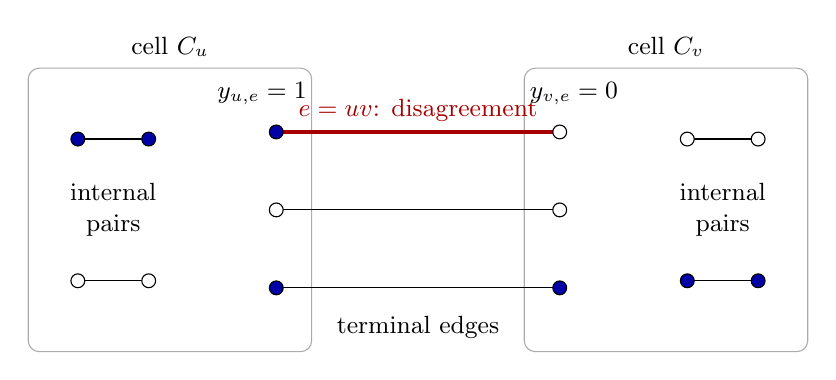
\begin{tikzpicture}[x=.9cm,y=.9cm,font=\small]
 \tikzset{bit/.style={circle,draw,minimum size=5pt,inner sep=0pt},
  one/.style={bit,fill=blue!65!black},zero/.style={bit,fill=white}}
 \draw[rounded corners,gray!65] (0,0) rectangle (4,4);
 \draw[rounded corners,gray!65] (7,0) rectangle (11,4);
 \node at (2,4.3) {cell $C_u$};
 \node at (9,4.3) {cell $C_v$};
 \draw (.7,3)--(1.7,3) (.7,1)--(1.7,1);
 \draw (9.3,3)--(10.3,3) (9.3,1)--(10.3,1);
 \node[one] at (.7,3) {}; \node[one] at (1.7,3) {};
 \node[zero] at (.7,1) {}; \node[zero] at (1.7,1) {};
 \node[zero] at (9.3,3) {}; \node[zero] at (10.3,3) {};
 \node[one] at (9.3,1) {}; \node[one] at (10.3,1) {};
 \node[align=center] at (1.2,2) {internal\\pairs};
 \node[align=center] at (9.8,2) {internal\\pairs};
 \draw[very thick,red!65!black] (3.5,3.1)--(7.5,3.1)
  node[midway,above] {$e=uv$: disagreement};
 \draw (3.5,2)--(7.5,2) (3.5,.9)--(7.5,.9);
 \node[one] at (3.5,3.1) {}; \node[zero] at (7.5,3.1) {};
 \node[zero] at (3.5,2) {}; \node[zero] at (7.5,2) {};
 \node[one] at (3.5,.9) {}; \node[one] at (7.5,.9) {};
 \node[above] at (3.3,3.35) {$y_{u,e}=1$};
 \node[above] at (7.7,3.35) {$y_{v,e}=0$};
 \node at (5.5,.35) {terminal edges};
\end{tikzpicture}

\caption{Part of the matching associated with two cells.  Filled vertices
belong to the cut and open vertices do not.  The restriction gives equal
bits to each internal pair, so only terminal edges can cross.  The
highlighted edge corresponds to a disagreement at an auxiliary edge
$e=uv$.  Only a few of the $d$ terminals and internal pairs are shown.}
\label{fig:matching-cells}
\end{figure}

\paragraph{A factorization and its Fourier approximation.}
Suppose that $A_n(\rho)$ has a PSD factorization of size at most
$2^t$.  Its entries are positive and at most $n$.
Lemma~\ref{lem:normalization} gives factors of size $r\le2^t$ with
\[
 \tr F_U\le n,\qquad \tr G_M\le r.
\]
Put $F(a)=F_{U(a)}$.  For any fixed local column data $m$, let
$\overline F_m(y)$ be the product-restricted average of $F$.
Equation~\eqref{eq:matching-realization} gives the exact identity
\begin{equation}\label{eq:matching-pairing}
 \tr\bigl(\overline F_m(y)G_{M(m)}\bigr)=f(y).
\end{equation}

Apply Theorem~\ref{thm:fourier-smoothing} with the local channels
above, the trace bound $B=n$, and
Equation~\eqref{eq:matching-local-smallness}.  It gives a choice of
$m$ and rectangular matrix functions $H_q$, indexed by
$q\in\Lambda^t$, such that
\begin{align}
 \overline F_m(y)&=\sum_q H_q(y)^{\mathsf T}H_q(y),
 \label{eq:matching-squares}\\
 \sum_{q,p}\lambda^{\dist(q,p)}\normF{\widehat H_{q,p}}^2
 &\le L^t\sqrt r\,n2^{t/2}.
 \label{eq:matching-fourier-bound}
\end{align}
Here $\Lambda$ is the character group on $d-1$ free bits, and
$\dist$ counts differing blocks.  Fix these data and set
$G=G_{M(m)}$.  By Equations~\eqref{eq:matching-pairing} and
\eqref{eq:matching-squares},
\begin{equation}\label{eq:matching-full-squares}
 f(y)=\sum_q\normF{H_q(y)G^{1/2}}^2.
\end{equation}

Let $D=\lfloor\tau t\rfloor$.  In branch $q$, retain only the
Fourier coefficients at distance at most $D$ from $q$, writing
\[
 K_q(y)=\sum_{p:\,\dist(q,p)\le D}\widehat H_{q,p}\chi_p(y),
 \qquad
 f_*(y)=\sum_q\normF{K_q(y)G^{1/2}}^2.
\]
The sum of squared norms of the discarded matrices at any $y$ is
at most
\begin{align}
 E_t(y)^2
 &:=\sum_q\normF{(H_q(y)-K_q(y))G^{1/2}}^2\notag\\
 &\le L^t\sum_{q,p:\,\dist(q,p)>D}
                    \normF{\widehat H_{q,p}G^{1/2}}^2\notag\\
 &\le L^t r\lambda^{-\tau t}
              \bigl(L^t\sqrt r\,n2^{t/2}\bigr)\notag\\
 &\le n\left(\frac{4L^2}{\lambda^\tau}\right)^t
 \le n(4L)^{-2t}.
 \label{eq:matching-tail}
\end{align}
The first inequality is Cauchy--Schwarz over at most $L^t$
characters in each branch.  The second uses
$\normop G\le\tr G\le r$, Equation~\eqref{eq:matching-fourier-bound},
and the fact that an integer distance greater than $D$ is greater
than $\tau t$.  The last line uses $r\le2^t$ and
Equation~\eqref{eq:matching-lambda}.

The full stack in Equation~\eqref{eq:matching-full-squares} has norm
at most $\sqrt n$.  Expanding the difference of the squared norms
of that stack and its truncation, and then using
Equation~\eqref{eq:matching-tail}, gives
\begin{equation}\label{eq:matching-uniform-error}
 \norm{f-f_*}_\infty
 \le 2n(4L)^{-t}+n(4L)^{-2t}.
\end{equation}

\paragraph{The separating functional.}
In branch $q$, multiplication by the real character $\chi_q$
does not change any square.  It translates a retained frequency
$p$ to $p+q$, whose block degree is $\dist(p,q)\le D$.
This character translation is the elementary support-shifting
principle used in Fourier sums of squares
\cite{fsp-sparse}.
Consequently $f_*$ is a sum of squares of real functions of block
degree at most $D$, including after multiplication by the constant
matrix $G^{1/2}$.

Proposition~\ref{prop:parity-functional} therefore supplies a
functional $\mathcal D$ with
\[
 \mathcal D(f_*)\ge0,\qquad \mathcal D(f)=-\epsilon.
\]
On the other hand, its norm bound and
Equation~\eqref{eq:matching-uniform-error} give
\[
 |\mathcal D(f-f_*)|
 \le 2n4^{-t}+n(16L)^{-t}\longrightarrow0
\]
by Equation~\eqref{eq:matching-size}, since $k$ is fixed.
For sufficiently large $n$, this is smaller than $\epsilon$,
a contradiction.

We have excluded every factorization of size at most $2^t$.
For all sufficiently large $n$, Equation~\eqref{eq:matching-size}
also gives $t\ge n/(2k)$.  Thus
\[
 \rankpsd A_n(\rho)>2^t\ge2^{n/(2k)}.
\]
Taking $c=1/(2k)$ proves the theorem.  Only the final comparison
with $\epsilon=1-\rho$ makes the threshold depend on $\rho$.
\end{proof}

\appendix
\section{Uniform smoothing of matching averages}\label{sec:matching-smoothing}

This appendix proves an independent smoothing theorem for averages over
perfect matchings with prescribed numbers of edges between vertex cells.
The number of cells is fixed, but their sizes and the prescribed counts
may vary arbitrarily.  The conclusion holds even when the prescribed
table has very small probability.  Besides an operator-norm estimate,
we obtain a single polynomial that describes all the low-degree averages
at a given partition.

The proof uses the same comparison between a fourth moment and eigenspace
dimensions as Lemma~\ref{lem:local-averaging}.  Here the inputs are
functions of perfect matchings, and removing products of a bounded number
of edge indicators makes the relevant dimensions grow by an arbitrarily
large power of the number of vertices.

Fix a positive integer \(\ell\).  For even \(N\), let \(\mathcal X\)
be the perfect matchings on a fixed \(N\)-element vertex set, and let
\(\mathcal Z\) be the ordered partitions into cells of positive sizes
\(s_1,\ldots,s_\ell\), with \(\sum_us_u=N\).  Both spaces carry the
uniform probability measure.  The \emph{table} of a matching at a
partition records its internal edge counts \(t_{uu}\) and its edge
counts \(t_{uv}=t_{vu}\) between distinct cells.  A table is admissible
if its entries are nonnegative integers and
\begin{equation}\label{smooth:eq-table-degrees}
  2t_{uu}+\sum_{v\ne u}t_{uv}=s_u
  \qquad (1\le u\le\ell).
\end{equation}
These conditions suffice: allocate the required endpoints in each
cell, pair the allocated endpoints between cells, and match the
remaining vertices internally.

For an admissible table, define
\(T_t:L^2(\mathcal X)\longrightarrow L^2(\mathcal Z)\) by
\[
  (T_tf)(Z)=\E[\,f(M)\mid M\text{ has table }t\text{ at }Z\,].
\]
Let \(\mathcal P_d\) be the span of products of at most \(d\) edge
indicators \(x_e(M)=\mathbf1_{\{e\in M\}}\), including the constant,
and let \(\Pi_d\) be its orthogonal projection.

\begin{theorem}[Uniform smoothing]\label{thm:matching-smoothing}
For every fixed \(\ell\ge1\) and \(K>0\), there are an integer
\(d\ge1\) and \(N_0\) such that, for every even \(N\ge N_0\), every
positive integer cell-size vector summing to \(N\), and every admissible table,
\begin{equation}\label{smooth:eq-smoothing}
  \normop{T_t(I-\Pi_d)}\le N^{-K}.
\end{equation}
Moreover, for each fixed partition \(Z\) and function \(f\), the values
\((T_t\Pi_df)(Z)\), as \(t\) varies over all admissible tables, are
given by a single polynomial of total degree at most \(d\) in the
intercell counts \((t_{uv})_{u<v}\).
\end{theorem}

The approximation error in \eqref{smooth:eq-smoothing} is measured in
\(L^2(\mathcal Z)\), with respect to the uniform choice of partition.
We prove the analytic estimate by combining a polynomial bound on a
fourth moment with a lower bound on the dimensions of the permutation
representations outside \(\mathcal P_d\).  The polynomial assertion will
then follow from a direct containment count.

\subsection{The fourth moment}

\begin{lemma}\label{smooth:lem-fourth-moment}
Put \(a_\ell=\ell(\ell+1)+1\) and
\(b_\ell=2a_\ell+\ell^2\).  For every admissible table,
\begin{equation}\label{smooth:eq-fourth-moment}
  \tr\bigl((T_t^*T_t)^2\bigr)
  \le e^{2a_\ell}(N+1)^{b_\ell}.
\end{equation}
\end{lemma}

\begin{proof}
Write \(h=N/2\).  For a fixed matching, the number of partitions
giving it table \(t\) is
\[
 D_t=\frac{h!}{\prod_{u\le v}t_{uv}!}\,
                  2^{\sum_{u<v}t_{uv}},
 \qquad
 |\mathcal Z|=\frac{N!}{\prod_us_u!}.
\]
The first formula assigns cell types to the \(h\) edges and chooses
which endpoint occupies which cell for each intercell edge.
Permutation transitivity shows that the table probability is
\(p_t=D_t/|\mathcal Z|\), whether the matching or the partition is
fixed.  Thus the density kernel of \(T_t\), relative to the uniform
measures, is the table indicator divided by \(p_t\).

Let \(J(M,M')\) count partitions giving table \(t\) to both matchings.
The density kernel of \(\mathcal A=T_t^*T_t\) is consequently
\begin{equation}\label{smooth:eq-matching-kernel}
 \kappa(M,M')=\frac{|\mathcal Z|}{D_t^2}J(M,M'),
 \qquad
 \tr(\mathcal A^2)=\E_{M,M'}\kappa(M,M')^2,
\end{equation}
where \(M,M'\) are independent and uniform.

We first bound this kernel using the alternating cycles of
\(M\cup M'\).  Define
\[
 \pi_u=\frac{s_u}{N},\qquad
 \gamma_{uu}=\frac{2t_{uu}}N,\qquad
 \gamma_{uv}=\frac{t_{uv}}N\quad(u\ne v).
\]
The array \(\gamma\) is symmetric, has total sum one, and has row sums
\(\pi\).  For a probability vector or array write
\(H(p)=-\sum_jp_j\log p_j\), with \(0\log0=0\).  The factorial
formulas imply
\begin{equation}\label{smooth:eq-table-entropy}
 \log\frac{D_t^2}{|\mathcal Z|}
 =N\bigl(H(\gamma)-H(\pi)\bigr)+\Delta,
 \qquad
 \Delta\ge-a_\ell\bigl(1+\log(N+1)\bigr).
\end{equation}
To check the remainder uniformly, including zero table entries, put
\(R_0=0\) and
\(R_j=\log(j!)-j\log j+j\) for \(j\ge1\).
Integral comparison gives \(0\le R_j\le1+\log(j+1)\), and direct
substitution gives
\[
 \Delta=2R_h-2\sum_{u\le v}R_{t_{uv}}-R_N+\sum_uR_{s_u}.
\]
There are \(\ell(\ell+1)/2\) unordered table entries, proving the
stated lower bound.  In the leading term, splitting each unordered
off-diagonal frequency into two ordered frequencies accounts for
the power of two in \(D_t\).

Retain doubled edges in \(M\cup M'\), so that its components are
alternating cycles, including cycles of length two.  Orient each
cycle and write \(c=c(M,M')\) for their number.  The matrix
\(W_{uv}=\gamma_{uv}/\pi_u\) is nonnegative and stochastic.  Give a
vertex coloring by \(1,\ldots,\ell\) the weight obtained by
multiplying \(W_{uv}\) over the oriented edges, where \(u,v\) are
the tail and head colors.

Every coloring counted by \(J(M,M')\) has weight
\begin{equation}\label{smooth:eq-table-color-weight}
 \exp\{-N(H(\gamma)-H(\pi))\}.
\end{equation}
Indeed, each vertex occurs once as a tail, so the denominator is
\(\prod_u\pi_u^{s_u}\).  The two matchings together contribute
\(2t_{uv}\) edges of each unordered type.  Symmetry of \(\gamma\)
makes their orientations irrelevant, and the numerator is
\(\prod_{u\le v}\gamma_{uv}^{2t_{uv}}\), with zero exponents omitted.
These expressions give \eqref{smooth:eq-table-color-weight}; no counted
coloring uses a zero entry of \(\gamma\).

For a cycle of length \(a\), the sum of weights over all its colorings
is \(\tr(W^a)\le\ell\).  Summing over all vertex colorings therefore
bounds the total weight of the colorings counted by \(J\) by
\(\ell^c\).  Equations \eqref{smooth:eq-matching-kernel}--\eqref{smooth:eq-table-color-weight}
yield
\begin{equation}\label{smooth:eq-matching-kernel-bound}
 \kappa(M,M')\le e^{a_\ell}(N+1)^{a_\ell}\ell^{c(M,M')}.
\end{equation}

It remains to average the cycle factor.  Set \(b=\ell^2\).  The
number \(b^c\) counts colorings that are constant on every edge of
both matchings.  Fix \(M\), and suppose its \(h\) edges have color
multiplicities \(j_1,\ldots,j_b\), summing to \(h\).  Averaging the
number of such colorings over \(M'\) gives the contribution
\[
 \frac{h!}{\prod_i j_i!}
 \frac{\prod_i(2j_i-1)!!}{(2h-1)!!}
 =\frac{\prod_i\binom{2j_i}{j_i}}{\binom{2h}{h}}
 \le1,
\]
where \((-1)!!=1\).  For the inequality, partition a \(2h\)-element
set into blocks of sizes \(2j_i\): the numerator counts only those
\(h\)-element subsets taking \(j_i\) elements from each block.
There are at most \((h+1)^b\) possible multiplicity vectors.  Hence
\(\E\ell^{2c}\le(h+1)^{\ell^2}\).  Squaring
\eqref{smooth:eq-matching-kernel-bound} and using
\eqref{smooth:eq-matching-kernel} proves \eqref{smooth:eq-fourth-moment}.
\end{proof}

\subsection{Dimensions outside the edge-product span}

The fourth-moment bound alone does not make the operator small.
The additional fact is that each eigenspace of the compression of
\(T_t^*T_t\) to \(\mathcal P_d^\perp\) is invariant, and every nonzero
such space has large dimension.  Here we use the standard
representation theory of the symmetric group over the complex
numbers: irreducibles are indexed by Young diagrams, restriction
from \(S_N\) to \(S_{N-1}\) deletes a corner box, and dimensions count
standard Young tableaux.  The one-row and one-column diagrams give
the trivial and sign representations.  These facts, including the
branching rule, are described in
\cite[Theorem~5.8, Section~6, and Corollary~7.1]{vershik-okounkov}.

\begin{lemma}\label{smooth:lem-dimension}
For each fixed integer \(d\ge1\) and all sufficiently large \(N\),
every irreducible constituent of the complexification of
\(\mathcal P_d^\perp\) has dimension at least
\[
 c_dN^{d/2},\qquad c_d=\frac1{2^dd!}.
\]
\end{lemma}

\begin{proof}
Fix a set of \(d\) vertices, and let \(G\cong S_{N-d}\) permute the
other vertices.  A \(G\)-orbit of matchings is determined by the
internal matching \(F\) on the fixed vertices: a permutation can
first align the outside partners of all unmatched fixed vertices
and then align the remaining outside edges.  The orbit indicator is
\[
 \prod_{e\in F}x_e
 \prod_{\substack{e\text{ on the fixed vertices}\\e\notin F}}(1-x_e).
\]
On expansion, a nonzero monomial uses only disjoint edges among
those \(d\) vertices, and therefore at most \(\lfloor d/2\rfloor\)
edge indicators.  All \(G\)-invariant functions consequently belong
to \(\mathcal P_d\).

If a Young diagram has first row of length at least \(N-d\), the
branching rule gives a \(G\)-fixed vector in its irreducible
representation: remove corner boxes until only a row of size
\(N-d\) remains.  Such a representation cannot occur in
\(\mathcal P_d^\perp\), since any such copy would provide a nonzero
\(G\)-fixed vector there.

A first column of length at least \(N-d\) similarly gives a vector
transforming by the sign character of \(G\).  No nonzero matching
function has this transformation law when \(N>2d\).  In fact,
every matching then contains an edge entirely outside the fixed
vertices; transposing its endpoints belongs to \(G\), fixes that
matching, and reverses the sign of the function.  The function must
vanish at every matching.  Thus a diagram occurring in
\(\mathcal P_d^\perp\) has both first row and first column shorter than
\(N-d\).

Let \(\lambda\) be any remaining diagram.  The product of its first
row and first column lengths is at least \(N\).  Transpose if
necessary so that its first row has length \(b\ge\sqrt N\);
transposition preserves the number of standard tableaux.  Retain
that row and a Young subdiagram of exactly \(d\) boxes below it.
Such a subdiagram exists because \(N-b\ge d\).

For large \(N\), we have \(b\ge2d\).  Put \(1,\ldots,d\) into the
first \(d\) positions of the top row.  Choose any \(d\) of the
remaining \(b\) labels \(d+1,\ldots,b+d\) for the lower boxes, fill
those boxes in a fixed standard order, and put the unused labels
increasingly into the rest of the top row.  Each lower box is in
one of the first \(d\) columns, so the resulting tableau is
standard.  The \(\binom bd\) choices give distinct tableaux of this
subdiagram.  Each extends to \(\lambda\) by adding the remaining
boxes along a fixed corner-addition chain with successively larger
labels.  The dimension \(f^\lambda\) therefore satisfies
\[
 f^\lambda\ge\binom bd
 \ge\frac{b^d}{2^dd!}
 \ge c_dN^{d/2},
\]
as required.
\end{proof}

\subsection{From moments to smoothing, and from products to polynomials}

\begin{proof}[Proof of Theorem~\ref{thm:matching-smoothing}]
Complexification does not change operator norms.  The operator
\(\mathcal A=T_t^*T_t\) commutes with vertex permutations, since
\(T_t\) intertwines their actions on matchings and partitions.
The projection \(Q=I-\Pi_d\) also commutes with permutations,
because \(\mathcal P_d\) is invariant.  The compression
\(B=Q\mathcal A Q\), acting on \(\mathcal P_d^\perp\), is therefore
positive semidefinite and equivariant.  Moreover,
\[
 \tr(B^2)\le\tr(\mathcal A^2),\qquad
 \normop{B}=\normop{T_tQ}^2.
\]
The first inequality is contraction of the Hilbert--Schmidt norm
under orthogonal compression and does not require \(Q\) and
\(\mathcal A\) to commute.

If \(B\ne0\), its largest-eigenvalue eigenspace is invariant and
contains an irreducible constituent.  Lemma~\ref{smooth:lem-dimension}
and the fourth-moment bound give
\[
 c_dN^{d/2}\normop{T_tQ}^4
 \le e^{2a_\ell}(N+1)^{b_\ell}.
\]
The same inequality holds if \(B=0\).  Choose \(d\) so that
\(d/2>b_\ell+4K\).  For all sufficiently large \(N\), this proves
\eqref{smooth:eq-smoothing}, uniformly in the sizes and the table.

To prove the polynomial assertion, fix a partition and a generating
product of edge indicators.  Repeated indicators may be removed,
and a product containing two distinct incident edges vanishes.
Otherwise the specified edges form a partial matching.  Let
\(m_{uv}\) be its type counts and let
\[
 a_u=2m_{uu}+\sum_{v\ne u}m_{uv}
\]
be the number of its endpoints in cell \(u\).  The probability
that a matching with table \(t\) contains these specified edges is
\begin{equation}\label{smooth:eq-containment}
 \frac{2^{\sum_um_{uu}}\prod_{u\le v}(t_{uv})_{m_{uv}}}
      {\prod_u(s_u)_{a_u}},
 \qquad
 (z)_j=z(z-1)\cdots(z-j+1),\quad (z)_0=1.
\end{equation}
Indeed, apply a uniform cell-preserving vertex permutation to any
one matching with table \(t\).  This is uniform over all such
matchings by transitivity.  The denominator counts injections of
the specified endpoint lists, while the numerator chooses distinct
edges of each type and the two orientations of each internal edge.
The denominator is positive because \(a_u\le s_u\).
If \(t_{uv}<m_{uv}\) for any type, its falling factorial is zero,
as required.

The numerator of \eqref{smooth:eq-containment} has total degree equal to
the number of specified edges.  Equation~\eqref{smooth:eq-table-degrees}
expresses every \(t_{uu}\) as an affine function of the intercell
counts.  Thus the containment probability is a polynomial of the
required degree in those counts.  By linearity this holds for
\(\Pi_df\); its expansion in edge products is fixed independently
of \(t\), so the resulting polynomial works simultaneously for all
admissible tables.
\end{proof}


With three cells, the table is determined by its three intercell edge counts.

\begin{corollary}[Three-cell smoothing]\label{cor:three-cell}
For every fixed $K>0$, there are an integer $d\ge1$ and $N_0$ with the following property. Let $N\ge N_0$ be even, and let $a,b,c$ be positive integers summing to $N$. For a uniform ordered partition into cells of these sizes, prescribe $x,y,z$ edges between the first and second, first and third, and second and third cells, respectively. Assume that $x,y,z$ are nonnegative integers and that
\[
 a-x-y,\qquad b-x-z,\qquad c-y-z
\]
are nonnegative even integers. Let $T_{x,y,z}$ average functions on perfect matchings subject to these counts, and let $\Pi_d$ project onto the edge-product span of degree at most $d$, using uniform measures as above. Then
\[
 \normop{T_{x,y,z}(I-\Pi_d)}\le N^{-K}
\]
uniformly in all the sizes and admissible triples. For every fixed partition and matching function $f$, the values $T_{x,y,z}\Pi_df$ are given by one polynomial of total degree at most $d$ in $(x,y,z)$ across all admissible triples.
\end{corollary}

\begin{proof}
Apply Theorem~\ref{thm:matching-smoothing} with $\ell=3$, intercell counts $t_{12}=x$, $t_{13}=y$, $t_{23}=z$, and internal counts $(a-x-y)/2$, $(b-x-z)/2$, $(c-y-z)/2$.
\end{proof}

\bibliographystyle{plain}
\bibliography{refs}
\end{document}
